\documentclass{article}
\usepackage[utf8]{inputenc}
\usepackage[a4paper]{geometry}
\usepackage[myheadings]{fullpage}
\usepackage[english]{babel}
\usepackage[T1]{fontenc}
\usepackage{sectsty}
\usepackage{appendix}
\usepackage{fancyhdr}
\usepackage{lastpage}
\usepackage{setspace}
\usepackage{amsmath}
\usepackage[yyyymmdd]{datetime}
\usepackage{longtable}
\usepackage{graphicx}
\usepackage[table, xcdraw]{xcolor}
\usepackage{pgfplots}
\usepackage{tikz}
\usepackage[
    backend=bibtex,
    style=numeric,
    sorting=none
]{biblatex}
\usepackage{hyperref}
\addbibresource{bibliography.bib}

\renewcommand{\dateseparator}{-}
\makeatletter
\renewcommand{\paragraph}{\@startsection{paragraph}{4}{0ex}%
    {-3.25ex plus -1ex minus -0.2ex}%
    {1.5ex plus 0.2ex}%
    {\normalfont\normalsize\bfseries}}
\makeatother

\pgfplotsset{compat=1.16}
\usetikzlibrary{positioning}

\onehalfspacing

\pagestyle{fancy}
\fancyhf{}
\setlength\headheight{15pt}
\fancyhead[L]{21963144}
\fancyhead[R]{UWA}
\fancyfoot[R]{Page \thepage{} of \pageref{LastPage}}
\sectionfont{\scshape}

\newcommand{\HRule}[1]{\rule{\linewidth}{#1}}

\title{\normalsize \textsc{Masters Dissertation}
        \\ [1.5cm]
        \HRule{0.5pt} \\
        \LARGE \textbf{\uppercase{Implementation of \(N\)-detectors in a gravitational wave detection pipeline}}
        \HRule{2pt} \\ [0.5cm]
        \normalsize \date{\today} \vspace*{2\baselineskip}}

\author{Thomas Hill Almeida (21963144)\thanks{Software Engineering, University of Western Australia}\\
\small{Supervisors: Prof. Linqing Wen\thanks{Department of Physics, University of Western Australia}, Qi Chu\footnotemark[2]}}
\date{}

\begin{document}
\maketitle{}
\newpage{}
\tableofcontents{}
\newpage{}

\begin{minipage}[t]{0.6\textwidth}
    \centering
    \section*{} \label{sec:abstract}
    % TODO: Write abstract
\end{minipage}

\section{Introduction} \label{sec:introduction}

Gravitational waves have been postulated to exist since Albert Einstein's publication of his general theory of relativity, as massive accelerating objects would cause `ripples' in the curvature of spacetime \cite{ligo_einstein}.
Direct detection of gravitational waves, however, remained beyond the reach of the scientific community until 2015, when the Laser Interferometric Gravitational-Wave Observatory (LIGO \cite[see][]{LIGO}) reported an observation on the 14th of September \cite{FirstDetectionPaper, DetectionWeb}.

Due to their design, the detectors in use for gravitational wave detection have a significant amount of noise from other sources, whilst the gravitational waves themselves have very weak signals.
As such, a large amount of data processing must be done to the outputs produced by the detectors in order to filter and extract any possible gravitational waves.
These data processors are known as ``pipelines'', and have historically been created by research groups that are a part of the LIGO Scientific Collaboration (LSC \cite[see][]{LSC}), and are used throughout observation runs for real-time data analysis.
\\

The Summed Parallel Infinite Impulse Response (SPIIR \cite[see][]{spiir}) pipeline, based on the SPIIR method originally implemented by Shaun Hooper in 2012, uses a number of IIR (infinite impulse response) filters to approximate possible gravitational wave signals for detection \cite{SPIIRCreate}.
\cite{SPIIRGPU2018} states that the output of the \(i\)th IIR filter can be expressed with the equation:
\begin{equation}
    y^i_k = a^i_1y^i_{k-1} + b^i_0x_{k-d_i},
\end{equation}
\\
where \(a^i_1\) and \(b^i_0\) are coefficients, \(k\) is time in a discrete form and \(x_{k-d_i}\) denotes input with some time delay \(d_i\).
After summing the output of the filters, the resulting signal undergoes coherent post-processing (see section \ref{sec:discuss:analysis} and \cite[chapter 4]{ChuThesis}) to determine the likelihood of an event having occurred.

The pipeline is currently thought to be the fastest of all existing pipelines, is the only pipeline that implements coherent search, and has participated in every observation run since November 2015, successfully detecting most events that were seen in more than one detector.

The SPIIR pipeline uses GStreamer, a library for composing, filtering and moving around signals, in addition to the GStreamer LIGO Algorithm Library (\texttt{gstlal}) \cite{gstlal}.
After receiving data from the detectors, the pipeline performs data conditioning and data whitening, followed by the usage of the IIR filters.
The data is then combined for post-processing, where events are given sky localization and then inserted into the LIGO event database \cite{SPIIRGPU2018}.

The structure of the SPIIR pipeline can be seen in figure \ref{fig:spiir_structure}.

\begin{figure}
    \label{fig:spiir_structure}
    \centering
    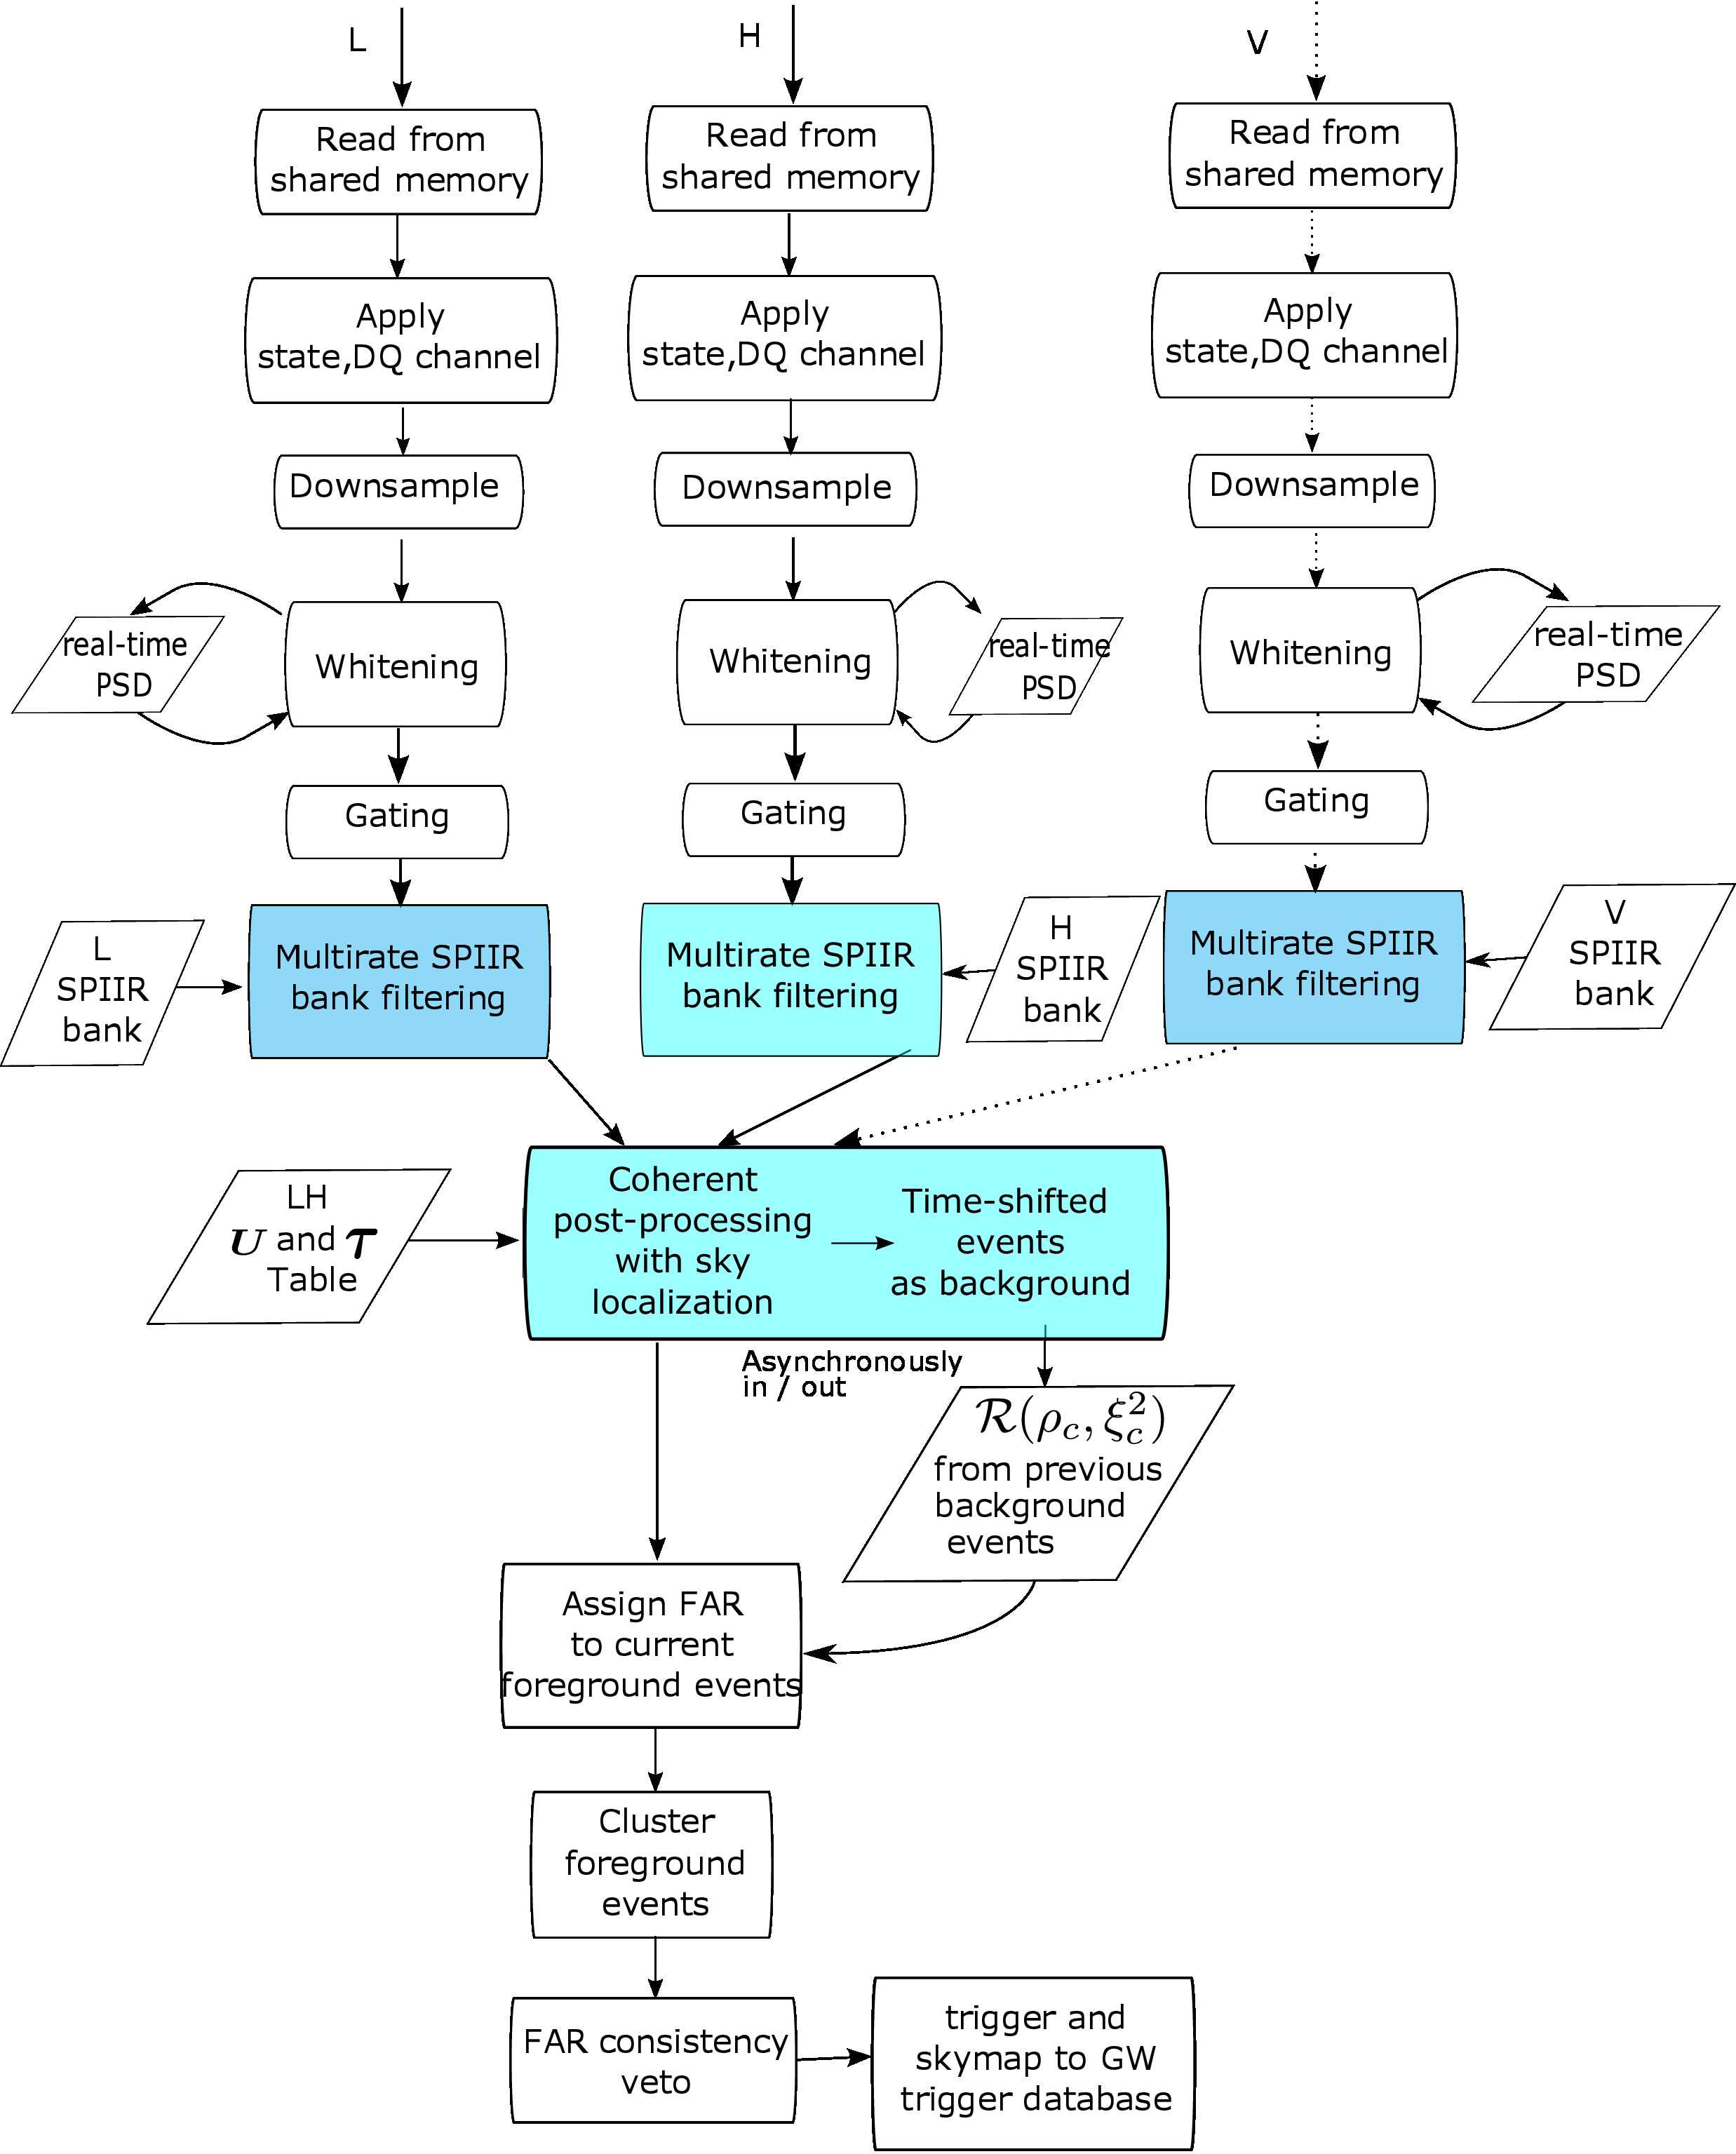
\includegraphics[scale=0.18]{../seminar-presentation/online_xdet.jpg}
    \caption{The structure of the SPIIR pipeline}
\end{figure}

\subsection{Research Aims} \label{sec:introduction:aims}

At the time of the start of this research, the SPIIR pipeline supported the use of two or three detectors for gravitational wave detection \textemdash{} the two American LIGO detectors and the Italian Virgo detector \textemdash{} although additional interferometers are likely to be introduced soon.
This presents several issues with the existing pipeline design.

As with many of the other gravitational wave detection pipelines, providing support for additional detectors is a significant undertaking for the development team, with many hours of work and testing that need to be completed.
As the number of available interferometers continues to grow, development work that could be spent on improving the optimisation, precision, or accuracy of the pipeline would instead have to be spent allowing for those detectors to be used.

Thus, this dissertation aims to layout the design and implementation work done to provide the SPIIR pipeline with the ability to support any number of detectors (\(N\)-detectors).
\\

Section \ref{sec:lit_review} shall explore the existing literature on the implementation of \(N\)-detectors in other gravitational wave detection pipelines, in addition to exploring CUDA and complexity analysis, two tools that will be used in the analysis of the final design.
Section \ref{sec:design_process} will look at the existing pipeline structure and its deficiencies for implementing \(N\)-detectors.
It will also determine any constraints a design for implementing \(N\)-detectors would have, and will provide a framework for evaluating the success of the resulting design.
The final design will be presented in section \ref{sec:final_design}, and will explore the implementation details of the design and how it interacts with the existing programming interface that SPIIR provides.
A discussion about the implications of this design will be done in section \ref{sec:discuss}, with additional research on those implications being presented there.
Finally, section \ref{sec:further_work} will provide some suggestions for future research that can be based on this research.

\section{Literature Review} \label{sec:lit_review}

This section explores the existing research that is relevant to this project.
Section \ref{sec:lit_review:pipelines} shall explore the implementations that other gravitational wave detection pipelines have used to deal with with a growing number of detectors in their algorithms and interfaces, whilst section \ref{sec:lit_review:cuda} will explore the computational model of CUDA, the library that SPIIR uses for parallelism.
Finally, section \ref{sec:lit_review:par_comp_analysis} shall explore the literature of parallel complexity analysis, which will allow for the later analysis of the pipeline in section \ref{sec:discuss:analysis}.

\subsection{\(N\)-detector work in other gravitational wave detection pipelines} \label{sec:lit_review:pipelines}

There are, of course, other gravitational wave detection pipelines that may also have to consider the issue of dealing with a growing number of detectors.
As we are in the process of designing a new architecture to allow for any number of detectors to be used, it is well worth examining the methods that the other pipelines may use to shape our own design.

Most detection pipelines use a ``coincidence'' search to determine whether a gravitational wave event has occurred.
Coincidence search, as defined by \cite[chapter 3]{ChuThesis}, is a process which includes finding candidates for gravitational waves from individual detectors, identifying temporal coincidences and producing measures to rank candidate events.
In more simple terms, a coincidence search considers events which can be seen in a single detector, and then sanity checks that other detectors may have seen them at the same time.

In contrast, the SPIIR pipeline uses a ``coherent'' search to determine whether a gravitational wave event has occurred, using the maximum likelihood ratio principle to consider specific parameters of a potential signal \cite[chapter 4]{ChuThesis}.
As such, it is unlikely that all of the principles for dealing with additional detectors may translate directly to being able to be used for the SPIIR pipeline, as the method of search differs.
\\

PyCBC is one of the most well known toolkits for gravitational wave astronomy, and was one of the pipelines used in the original 2015 gravitational wave detection \cite{pycbc_home}.
From an examination of the codebase of the latest version of PyCBC \cite[October 2020]{pycbc}, it can be observed that the codebase itself makes no direct mention of detectors \textemdash{} instead it provides a generic \texttt{Detector} class as a wrapper around LALSuite's \cite{lalsuite} \texttt{LALDetector} structure for validation, which in turns provides utilities for returning information about the detector as well as methods for getting readings from it.

This allows PyCBC to provide an entirely generic gravitational wave searching algorithm library for any input detectors, although the algorithm only supports using two detectors at a time, providing that the detectors are in the LALSuite library.
Thus, we can note two things; for PyCBC to allow for additional detectors to be used, they simply update their dependency on the LALSuite library, and; PyCBC doesn't quite support \(N\)-detectors in the sense described in section \ref{sec:introduction:aims}, instead it allows for any supported detectors to be used in a two-detector search.
This means that whilst we cannot use PyCBC when considering how to support support any number of detectors within a gravitational-wave searching algorithm nor its outputs, we can use PyCBC to consider a programming interface with which to support other detectors.
\\

GstLAL is gravitational wave detection library, that exposes components of LALSuite \cite{lalsuite} as GStreamer elements for use in other analysis pipelines \textemdash{} including the SPIIR pipeline \textemdash{} as well as providing its own pipeline for processing raw signals from detectors into lists of gravitational wave candidates \cite{gstlal_docs}.
The GstLAL's pipeline hard-codes the detector names into both its inputs and its outputs, however the algorithm used for detection itself is actually generic on which detectors are used \cite{gstlal_paper, gstlal_coinc}.

This means that the process of adding support for detectors involves changing a number of different files, as well as modifying several internal data structures \cite{messick} \textemdash{} which means that whilst GstLAL does not support \(N\)-detectors.
\\

Thus any work done to design \(N\)-detector support for the SPIIR pipeline will be novel work.

\subsection{CUDA} \label{sec:lit_review:cuda}

CUDA \cite{CUDA} is an extension of the C++ programming language created by NVIDIA that allows for the development of GPU-accelerated applications.
In \cite{SPIIRGPU2018}, the SPIIR pipeline had multiple components rewritten in CUDA to take advantage of the high number of simultaneous threads available compared to CPUs.
As such, it is worth understanding the computational model of CUDA for the analysis of the SPIIR pipeline.

In CUDA, each individual sequence of instructions being executed is called a \textit{thread}.
By its nature, a highly-parallelised environment such as GPUs will run many individual threads, which are partitoned into \textit{warps}, a group of (typically 32) threads.
Warps are the smallest unit that GPUs schedule, and all threads in a warp must execute the same instruction -- although each thread maintains its own instruction pointer and can branch independently from the warp at a small performance cost.
The performance cost of branching within a warp means that a major optimization that does not affect computational complexity in CUDA can be simply reducing the number of branches.
Warps are further organised into thread blocks, which contain a small amount of fast memory shared between the threads in the block.
Blocks in CUDA are typically executed on the same Simultaneous Multiprocessor (SM).
The CUDA Programming Guide (\cite{CUDA_Guide}) states that the number of blocks and warps that can reside and be processed together on an SM depends on the number of registers and shared memory available on the SM, as well as on a CUDA defined maximum number of blocks and warps.

For the purpose of actual time-based computation, the maximum number of threads that can run at any given time is determined by a few factors of the CUDA runtime; the maximum number of resident warps per SM; the maximum number of resident threads per SM; the number of 32-bit registers per thread; the number of 32-bit registers per SM; the number of 32-bit registers per thread block; and the amount of shared memory in each of those divisions.
Thus, one major determining factor in any speed-up given by a CUDA operation can be determined by the ability to split the workload across threads and thread blocks such that the number of registers and used memory is well balanced across threads.

\subsection{Parallelised Complexity Analysis} \label{sec:lit_review:par_comp_analysis}

As the pipeline changes to accommodate additional detectors, it is important that the impact that this has on the pipeline's runtime is considered.
The SPIIR pipeline is designed to be as low latency as possible, and an asymptotic complexity analysis of components that may be impacted by the addition of new detectors allows for the measurement of the potential runtime cost of doing so.
The SPIIR pipeline has been parallelised using CUDA \cite{SPIIRGPU2018}, and thus determining the asymptotic complexity of components of the pipeline requires different considerations to that of a sequential program.
\\

According to \cite{CLRS_parallel}, the theoretical efficiency of a multi-threaded or parallelised algorithm can be measured using the metrics of `span', `work', `speed-up' and `parallelism', all of which should be considered in the context of a directed acyclic graph (DAG) of operations in the algorithm.
The \textit{\textbf{work}} of a parallelised computation is the total time to execute the entire computation sequentially on a single processor, and can be found by summing the total work of every vertex in the DAG.
An example of \textit{\textbf{work}} for a merge-sort like algorithm can be seen in figure \ref{fig:work}, which has a work of \(O(N\log{N})\).
In comparison, the \textit{\textbf{span}} of a parallelised computation is the maximum time taken to complete any path in the DAG.
An example of \textit{\textbf{span}} for a merge-sort like algorithm can be seen in figure \ref{fig:span}, which has a work of \(O(N)\).
It should be noted that the actual running time of a parallelised computation also depends on the number of processors available for computation and how they are allocated to perform different tasks in the DAG, and thus denoting the running time of parallelised computation on \(P\) processors as \(T_P\) is also common practice.
This leads to work being denoted at \(T_1\) (the time taken to run on a single processor) and span being denoted as \(T_\infty\) (the time taken on an infinite number of processors).
Another helpful metric is \textit{\textbf{speed-up}}, which shows how the algorithm scales with additional processors as \(S_P = \dfrac{T_1}{T_P}\).
We can also then define \textit{\textbf{parallelism}} as the maximum possible speed-up on an infinite number of processors, and thus as \(p = \dfrac{T_1}{T_\infty}\).

\begin{figure}[t]
    \centering
    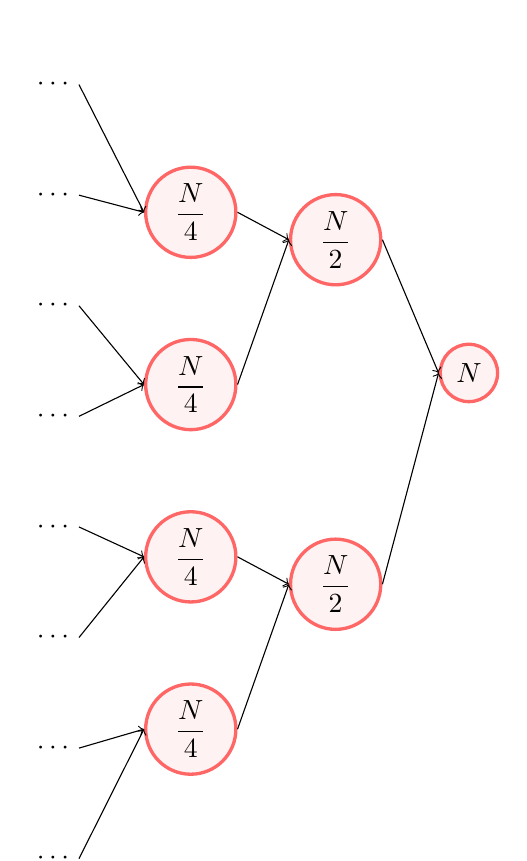
\begin{tikzpicture}[
        selectednode/.style={circle, text=black, draw=red!60, fill=red!5, very thick, minimum size=7mm},
        unselectednode/.style={circle, text=black, draw=green!60, fill=green!5, very thick, minimum size=7mm},
]
        \node[selectednode] (leftuu) {\(\dfrac{N}{4}\)};
        \node[selectednode] (leftul) [below=of leftuu] {\(\dfrac{N}{4}\)};
        \node[selectednode] (leftlu) [below=of leftul] {\(\dfrac{N}{4}\)};
        \node[selectednode] (leftll) [below=of leftlu] {\(\dfrac{N}{4}\)};
        \node[selectednode] (centeru) [below right=of leftuu, above right=of leftul] {\(\dfrac{N}{2}\)};
        \node[selectednode] (centerl) [below right=of leftlu, above right=of leftll] {\(\dfrac{N}{2}\)};
        \node[selectednode] (right) [above right=of centerl, below right=of centeru] {\(N\)};

        \node (luuu) [above left=of leftuu] {\(\cdots\)};
        \node (luul) [below left=of leftuu, below=of luuu] {\(\cdots\)};
        \node (lulu) [above left=of leftul, below=of luul] {\(\cdots\)};
        \node (lull) [below left=of leftul, below=of lulu] {\(\cdots\)};
        \node (lluu) [above left=of leftlu, below=of lull] {\(\cdots\)};
        \node (llul) [below left=of leftlu, below=of lluu] {\(\cdots\)};
        \node (lllu) [above left=of leftll, below=of llul] {\(\cdots\)};
        \node (llll) [below left=of leftll, below=of lllu] {\(\cdots\)};
        \draw[->] (luuu.east) -- (leftuu.west);
        \draw[->] (luul.east) -- (leftuu.west);
        \draw[->] (lulu.east) -- (leftul.west);
        \draw[->] (lull.east) -- (leftul.west);
        \draw[->] (lluu.east) -- (leftlu.west);
        \draw[->] (llul.east) -- (leftlu.west);
        \draw[->] (lllu.east) -- (leftll.west);
        \draw[->] (llll.east) -- (leftll.west);
        \draw[->] (leftuu.east) -- (centeru.west);
        \draw[->] (leftul.east) -- (centeru.west);
        \draw[->] (leftlu.east) -- (centerl.west);
        \draw[->] (leftll.east) -- (centerl.west);
        \draw[->] (centeru.east) -- (right.west);
        \draw[->] (centerl.east) -- (right.west);
    \end{tikzpicture}
    \caption{An example of calculating work for a merge-sort like algorithm. Summed nodes are in red.\label{fig:work}}
\end{figure}

\begin{figure}[t]
    \centering
    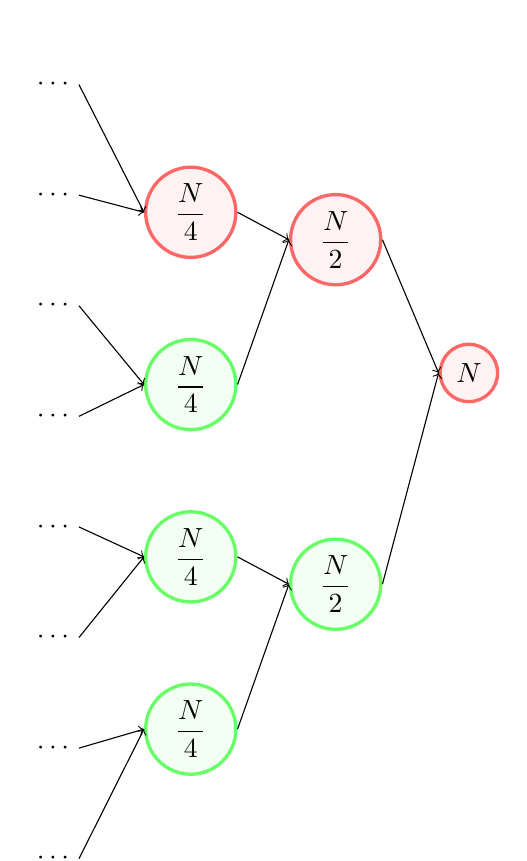
\begin{tikzpicture}[
        selectednode/.style={circle, text=black, draw=red!60, fill=red!5, very thick, minimum size=7mm},
        unselectednode/.style={circle, text=black, draw=green!60, fill=green!5, very thick, minimum size=7mm},
]
        \node[selectednode] (leftuu) {\(\dfrac{N}{4}\)};
        \node[unselectednode] (leftul) [below=of leftuu] {\(\dfrac{N}{4}\)};
        \node[unselectednode] (leftlu) [below=of leftul] {\(\dfrac{N}{4}\)};
        \node[unselectednode] (leftll) [below=of leftlu] {\(\dfrac{N}{4}\)};
        \node[selectednode] (centeru) [below right=of leftuu, above right=of leftul] {\(\dfrac{N}{2}\)};
        \node[unselectednode] (centerl) [below right=of leftlu, above right=of leftll] {\(\dfrac{N}{2}\)};
        \node[selectednode] (right) [above right=of centerl, below right=of centeru] {\(N\)};

        \node (luuu) [above left=of leftuu] {\(\cdots\)};
        \node (luul) [below left=of leftuu, below=of luuu] {\(\cdots\)};
        \node (lulu) [above left=of leftul, below=of luul] {\(\cdots\)};
        \node (lull) [below left=of leftul, below=of lulu] {\(\cdots\)};
        \node (lluu) [above left=of leftlu, below=of lull] {\(\cdots\)};
        \node (llul) [below left=of leftlu, below=of lluu] {\(\cdots\)};
        \node (lllu) [above left=of leftll, below=of llul] {\(\cdots\)};
        \node (llll) [below left=of leftll, below=of lllu] {\(\cdots\)};
        \draw[->] (luuu.east) -- (leftuu.west);
        \draw[->] (luul.east) -- (leftuu.west);
        \draw[->] (lulu.east) -- (leftul.west);
        \draw[->] (lull.east) -- (leftul.west);
        \draw[->] (lluu.east) -- (leftlu.west);
        \draw[->] (llul.east) -- (leftlu.west);
        \draw[->] (lllu.east) -- (leftll.west);
        \draw[->] (llll.east) -- (leftll.west);
        \draw[->] (leftuu.east) -- (centeru.west);
        \draw[->] (leftul.east) -- (centeru.west);
        \draw[->] (leftlu.east) -- (centerl.west);
        \draw[->] (leftll.east) -- (centerl.west);
        \draw[->] (centeru.east) -- (right.west);
        \draw[->] (centerl.east) -- (right.west);
    \end{tikzpicture}
    \caption{An example of calculating span for a merge-sort like algorithm. Summed nodes are in red.\label{fig:span}}
\end{figure}

Using the above definitions, we can re-derive several laws that provide lower bounds on the running time of \(T_P\).

In one step, a computer with \(P\) processors can do \(P\) units of work, and thus in \(T_P\) time can perform \(PT_P\) units of work.
As the total work to be done as per above is \(T_1\), the \textit{\textbf{work law}} states that \cite{CLRS_parallel}:

\begin{equation} \label{eq:work_law}
    T_P \geq \dfrac{T_1}{P}.
\end{equation}

It is also evident that a computer with \(P\) processors cannot run any faster than a computer with an infinite number of processors, as the computer with an infinite number of processors can emulate a computer with \(P\) processors by using a subset of its processors, leading to the \textit{\textbf{span law}} \cite{CLRS_parallel}:

\begin{equation} \label{eq:span_law}
    T_P \geq T_\infty.
\end{equation}

It is also useful to use the metrics of `cost' and `efficiency' when analysing parallel algorithms \cite{brent}.
The \textit{\textbf{cost}} of a parallel algorithm is minimised when all of processors are used at every step for useful computation and thus can be defined as \(C_P = P\times{T_P}\).
\textit{\textbf{Efficiency}} is closely related to cost and describes speed-up per processor and can be defined as:

\begin{equation} \label{eq:efficiency}
    e_P = \dfrac{S_P}{P} = \dfrac{T_1}{C_P}.
\end{equation}

Another helpful theorem for analysis is \textit{\textbf{Brent's Theorem}}, which states that for an algorithm that can run in parallel on \(N\) processors can be executed on \(P < N\) processors in a time of approximately \cite{BrentsLaw}

\begin{equation} \label{eq:brents_law}
    T_P \leq T_N + \dfrac{T_1-T_N}{P}.
\end{equation}

This can be approximated with the upper bound of \(O(\dfrac{T_1}{P} + T_N)\) \cite{brent}.

Determining the span, work, parallelism, efficiency and cost, and examining the application of Brent's theorem to the computations at hand will allow us to analyse the computational complexity of the SPIIR pipeline.

\section{Design process} \label{sec:design_process}

This section aims to layout and discuss the design process used to arrive at the final design of the \(N\)-detector implementation.
Section \ref{sec:design_process:constraints} will discuss the various design constraints that should be factored in any design implementation, and section \ref{sec:design_process:tools} will discuss the tools used throughout the design process.
The code sections that will be impacted by the implementation will be explored in section \ref{sec:design_process:code}, and a framework for evaluating the success of the implementation will be discussed in section \ref{sec:design_process:criteria}.

\subsection{Design Constraints} \label{sec:design_process:constraints}
% Description of the constraints imposed on the design

In the process of designing any system or any modifications thereof, constraints on that design must be considered and factored in.
This section aims to lay out and discuss the various design constraints that should be imposed on any final design.

The below constraints are ordered in importance.

\begin{itemize}
    \item \textbf{The output table format should be unchanged}\\
        Events that are detected by the SPIIR pipeline are uploaded to the gravitational-wave candidate event database (GraceDB) using a unified table format to represent event data \cite{gracedb}.
        It is of critical importance that the SPIIR pipeline is still able to interact with GraceDB so that it can continue to have detected events considered by the wider gravitational-wave community.
    \item \textbf{Adding new detectors should be able to be done by a non-technical individual}\\
        The wider gravitational-wave detection community is largely composed of physicists as opposed to software engineers.
        As such, any changes to the number of detectors are likely to be able to be best tested by non-technical members of the gravitational-wave community, as the expertise to ensure that the values output by the pipeline are correct are more likely to come from physicists.
        Any design for \(N\)-detector support should ensure that the process of adding detectors should be easy enough to be completed and tested by a non-technical individual.
    \item \textbf{The external interface of the pipeline should not change}\\
        There are many developers and scientists that are using the existing SPIIR pipeline and use customised scripts that automate gravitational wave searches.
        The ability to support \(N\)-detectors should be a largely internal change, without needing to modify the way that other users interact with the pipeline and force modifications to existing search scripts.
    \item \textbf{Individual detectors should still be exposed in Python code}\\
        There are several reasons for this constraint to be factored into any implementation.
        First, exposing individual detectors in the Python code allows for easier programming debugging of any values that may be incorrect, as the values of each detector would be immediately evident by the variable names instead of having be indirectly referenced by knowledge of the data structure used to hold the group of detectors.
        In addition, the Python code that interacts with GraceDB iterates through the list of detectors and uses the individual detector names to collect the data required for each event.
        By exposing individual detectors to the Python code, none of the code that interacts with GraceDB would need to change.
\end{itemize}

\subsection{Employed tools} \label{sec:design_process:tools}
% Description of any tools employed

\subsection{Relevant code} \label{sec:design_process:code}
% Discussion of relevant code sections or requirements

\subsection{Evaluation criteria} \label{sec:design_process:criteria}
% Framework for evaluating the success of the resulting design

\section{Final Design} \label{sec:final_design}

\subsection{Patches} \label{sec:final_design:patches}
% Description of the patches made

\subsection{Testing} \label{sec:final_design:testing}
% Testing of the design

\subsection{Evaluation} \label{sec:final_design:evaluation}
% Evaluation as per above

\section{Discussion} \label{sec:discuss}

\subsection{A complexity analysis of the parallel post-processing of the SPIIR pipeline} \label{sec:discuss:analysis}

Coherent post-processing was introduced in \cite{ChuThesis} by Qi Chu et al as an alternative to the coincidence post-processing used by all other pipelines (see section \ref{sec:lit_review:pipelines}).
\cite{ChuThesis} states that the multi-detector maximum log likelihood ratio to be equal to the coherent signal to noise ratio \(\rho{}^2_c\), which can be expressed as:

\begin{equation} \label{eq:coh_snr}
    \rho^2_c = \underset{\max\{A_{jk},\theta,t_{c},\alpha,\delta\}}{\ln \mathcal{L}_{NW}},
\end{equation}
\\
where \(A_{jk}\) describes the relative inclination of the detector to the source, \(\theta\) is the mass of the source, \(\alpha\) and \(\beta\) are the sky directions of the source and \(\mathcal{L}_{NW}\) is the network log likelihood network.

In \cite{ChuThesis}, the computational cost of the coherent search is estimated to be \(O(2N^3_dN_mN_p)\), where \(N_d\) is the number of detectors, \(N_m\) is the number of sets of IIR filters (called templates), and \(N_p\) is the number of potential sky locations.
Further optimizations were made to the pipeline in 2018 \cite{SPIIRGPU2018}, including moving to using GPU acceleration.
Whilst \cite{SPIIRGPU2018} discusses a number of constant time optimizations made to the pipeline, the computational cost of the overall process is not discussed.
In addition, \cite{SPIIRGPU2018} parallelised the pipeline, leading to additional potential changes to the potential overall cost.

\subsubsection{Motivation} \label{sec:discuss:analysis:motivation}

% TODO: Write motivation for complexity analysis. See seminar-presentation

\subsubsection{Maximum element reduction} \label{sec:discuss:analysis:reduce}

One of the more common operations in the SPIIR pipeline is the concept of a ``maximum element reduction''.
Reduction is the idea of taking some array of data and producing a single summary output from that array, whether it is the total sum of the array or the maximum value of the array and its index in the array as it is in this case.

\cite{reduction} discusses the computational complexity of reduction algorithms in a parallelised context, noting that the best complexity according to Brent's Law is \(O(\dfrac{N}{\log N})\) threads each doing \(O(\log N)\) sequential work, resulting in a total overall cost of \(O(\dfrac{N}{\log N}\times{\log N}) = O(N)\).

We can note from our own analysis, that the process of reduction can be parallelised by the use of a binary tree of operations, where each vertex in the binary tree combines the results of the two parent vertices.
In the case of determining the maximum of two numbers, each vertex is identical in the amount of work done, and thus we can determine each vertex to be a unit of work.
As there are \(N\) elements in the original array, we can note that the height of the binary tree is \(\log N\), and each level of the binary tree has \(N_l/2\) vertices, thus the total number of vertices in the binary tree is \(\sum_{i=0}^{\log N}{2\times{i}} = N\).
Using this information, we can determine that the \textit{\textbf{work}} of a parallelised reduction is \(T_1 = O(N\times1) = O(N)\), and that the \textit{\textbf{span}} of the reduction is \(T_\infty = O(\log N \times {1}) = O(\log N)\).
Thus, the \textit{\textbf{parallelism}} of the reduction is:

\[
    p = \dfrac{N}{\log N}.
\]

Using the span and work laws, we can observe that any algorithm using the above method is bounded by the inequalities \(O(\log N) \leq T_P, \dfrac{O(N)}{P} \leq T_P\).
This means that best possible time complexity with \(P\) processors is \(O(\log N)\) (equation \ref{eq:span_law}).
We can determine the minimum number of processors required to achieve this runtime using the formula \(T_P = O(\log N) = \dfrac{O(N)}{P}\), which can be rearranged to
\[
    P = \dfrac{N}{\log N},
\]
thus the time complexity cannot improve past \(P = N/\log N\) processors.
We can also observe that using \(P = N/\log N\) processors gives a \textit{\textbf{cost}} of \(C_P = N\), which is identical to the sequential algorithm.
\\

Functions that include maximum element reduction will be denoted for clarity with \(M(x)\), where \(x\) is the size of the array being reduced.

\subsubsection{Determining the number of samples over a signal-to-noise threshold} \label{sec:discuss:analysis:peaks}

The coherent post-processing in SPIIR determines the number of samples over a signal-to-noise (SNR) threshold in order to not do more work than is required.
The function that is used for determining the number of samples over the threshold (\texttt{peaks\_over\_thresh}) is a sequential algorithm that runs on the CPU, and shall be analysed as such, although there is an alternative GPU-based implementation that is not used.

Initially, the function performs a maximum element reduction to get the maximum SNR from the combined IIR filters (templates) for each sample.
Recalling from section \ref{sec:discuss:analysis:reduce} that for maximum element reduction \(T_1 = O(N)\), and that this operation is performed \(S\) times, where \(S\) is the number of samples, we can determine that this initial reduction has a time complexity of \(O(ST)\), where \(T\) is the number of templates.

The function then determines the maximum SNR across the templates found from the previous step by stepping through every combination of samples and removing SNR samples that are using the same template and have a lower SNR, resulting in a step with a time complexity of \(O(S^2)\).

The function then determines the maximum overall SNR for the input samples (\(O(S)\)) and cycles through every maximum SNR to cluster maxima that are close together to be a single combined maximum.
The number of maxima is bounded by (\(O(\min\{S,T\})\)) as there cannot be more maxima than there are samples or templates.

This gives the overall function a time complexity of \(O(ST + S^2 + S + \min\{S,T\})\), which can be reduced to the dominating terms of:

\[
    O(ST + S^2).
\]

\subsubsection{Transposing the input matrices} \label{sec:discuss:analysis:transpose}

The full post-processing function requires that the input matrix is transposed for better memory access such that each row is a different template, and each column is a different sample.
To transpose the matrix, the GPU function \texttt{transpose\_matrix} is used, thus this should be analysed as a parallel algorithm.

The algorithm in use works by breaking the original array into tiles of size \(32\times32\), and then inserting the transpose of the tile into an output array.
The tiles are further broken down eight processors per row, so each thread does four copies.
We can conceptualise this as a DAG by observing that each tile does not depend on any other tile to be completed, and that each tile is composed of \(32\times8\) interdependent processors, each doing 4 units of work.

Using this observation, we can see that the \textit{\textbf{span}} of the algorithm is \(T_\infty = (32\times8)\times4 = O(1024) = O(1)\), and the \textit{\textbf{work}} is \(T_1 = O(ST)\), where \(S\) is the number of samples and \(T\) is the number of templates.
Thus, the \textit{\textbf{parallelism}} of the transpose is \(p = ST\).

Using the span and work laws (equations \ref{eq:span_law} and \ref{eq:work_law}), we can observe that the above method is bounded by the inequalities \(O(1) \leq T_P, \dfrac{O(ST)}{P} \leq T_P\).
Thus it can be determined that the best possible time complexity with \(P\) processors is bounded by ratio of available processors to the size of the transposed matrix (the work law).
This gives the function an overall time complexity of:

\[
    O(\dfrac{ST}{P}).
\]

\subsubsection{Determining the coherent correlation and statistical value of data points} \label{sec:discuss:analysis:coh_max_and_chisq_versatile}

The scoring metric of different templates and times is determined using coherent correlation and determining their statistical value using a chi squared-based distribution.
These scoring metrics are performed using the GPU function \texttt{ker\_coh\_max\_and\_chisq\_versatile}, and thus should be analysed as a parallelised function.

In this function, each block looks at a different SNR maximum (as discussed in section \ref{sec:discuss:analysis:peaks}) and splits the threads within the blocks for operations on that peak.

\paragraph{Determining the sky direction of the SNR maximum} \label{sec:discuss:analysis:skydir}

Initially, each thread within a block looks at a different sky direction and determines the total signal-to-noise ratio (SNR) by summing the SNR of each of the detectors at that given sky direction with the relevant detector arrival time offsets.
The time complexity for the calculation of SNR for a given time offset is \(O(D + D^2)\), where \(D\) is the number of detectors.
The maximum SNR for all the sky directions is then spread across each warp and placed into shared memory before being shared across every thread in the block, which is an application of the parallelised maximum element reduction function discussed in section \ref{sec:discuss:analysis:reduce}.
\\

Thus, the \textit{\textbf{span}} of determining the sky direction with the highest signal to noise ratio is \(T_\infty = O(D + D^2 + M_{T_\infty}(S))\) and the \textit{\textbf{work}} is \(T_1 = O(S(D + D^2) + M_{T_1}(S)\), where \(S\) is the number of sky directions and \(M(x)\) is the complexity of the parallelised maximum element reduction function.
We can further state that the \textit{\textbf{parallelism}} of this is equivalent to the number of sky directions, \(S + S/\log S\).

\paragraph{Calculating signal consistency statistics} \label{sec:discuss:analysis:stat}

After having determined the sky direction with the highest SNR for a given maximum, the function then calculates a signal-morphology based statistic \(\xi_D^2\) for each detector \(D\).
The statistic is a reduced \(\chi^2\) distribution with \(D\times2 - 4\) degrees of freedom and a mean value of \(1\), and is given in the discrete form by:

\begin{equation} \label{eq:statistic}
    \xi_D^2 = \frac{\sum_{j = -m}^{m} | \varrho_D[j] - \varrho_D[0] A_D[j]|^2}{\sum_{j = -m}^{m} (2 - 2|A_D[j]|^2)},
\end{equation}
where \(\varrho\) is the coherent SNR, \(A_D\) is the vector of the correlation of the given template with the output from the detector and \(2\times{m}\) is the number of samples.

The numerator of the statistic is calculated by splitting the number of samples between the threads of a block, followed by combining the results of the statistic across each warp and then each block.
The combination of the statistic across each warp and block is a modification of the parallelised maximum element reduction discussed in section \ref{sec:discuss:analysis:reduce} that uses addition instead of maximum as the combining binary function.
Thus the \textit{\textbf{span}} of calculating the statistic is \(T_\infty = O(D\times{M_{T_\infty}(N)})\) and its \textit{\textbf{work}} is \(T_1 = O(D\times{M_{T_1}(N)})\), where \(N\) is the number of samples.
We can then state that the \textit{\textbf{parallelism}} of calculating the statistic is equivalent to the parallelism of the reduction, \(O(N/\log N)\).

\paragraph{Generating time-shifted background noise statistics} \label{sec:discuss:analysis:background}

% Why do we regenerate the background noise for every peak? Other than where we output
% the background noise, there's no difference between any of the peaks
%
% Removing background noise generation from this function would increase the speed of
% this function by an order of magnitude
The function then performs a number of time shifts on background noise for use with the significance estimation.
The generation of a single background statistical variant is equal to the total work of the function so far, save that instead of using blocks for every peak, each warp looks at a different time shift.
Thus, whilst the theoretical time complexity does not change, the number of processors available is smaller, so the actual runtime each loop is approximately the warp size slower.

\paragraph{Overall computational cost} \label{sec:discuss:analysis:versatile_cost}

Overall, this function has a \textit{\textbf{span}} of \(T_\infty = 2(D + D^2 + M_{T_\infty}(S) + DM_{T_\infty}(N))\), and has \(T_1 = P(S(D + D^2) + M_{T_1}(S) + DM_{T_1}(N) + B(S(D + D^2) + M_{T_1}(S)))\) \textit{\textbf{work}}, where \(P\) is the number of SNR maxima and \(B\) is the number of times shifts made to background noise.

\subsubsection{Calculating heat skymaps} \label{sec:discuss:analysis:coh_skymap}

If the coherent SNR exceeds a threshold, the post-processing produces a skymap of the highest SNR in the GPU function \texttt{ker\_coh\_skymap}.

The function determines the highest maximum SNR by using the maximum element reduction technique discussed in section \ref{sec:discuss:analysis:reduce}.
Following this, the function re-performs the process discussed in section \ref{sec:discuss:analysis:skydir} with additional sky directions and without the reduction to generate the final skymap.

As such, this function has a \textit{\textbf{span}} of \(T_\infty = M_{T_\infty}(P) + D + D^2\) and total \textit{\textbf{work}} of \(T_1 = M_{T_1}(P) + S(D + D^2)\).

\subsubsection{Overall complexity} \label{sec:discuss:analysis:overall}

The total span and work of the coherent post-processing step in the SPIIR pipeline is the sum of the total spans and works of the internal functions.
Conversely, we cannot determine the overall parallelism as the post-processing step spans a number individual functions that can each be run with a different set of processors.
As the step to determine the number of peaks over a threshold (see section \ref{sec:discuss:analysis:peaks}) is sequential, we can consider its time complexity as contributing to both the span and work of the total pipeline.
Another thing to note is that the steps for determining the coherent correlation, statistic value and skymaps (sections \ref{sec:discuss:analysis:coh_max_and_chisq_versatile} and \ref{sec:discuss:analysis:skydir}) will be run for every detector.

With this in mind, we can determine that the \textit{\textbf{span}} of the post-processing is:

\[
    T_\infty = O(NT + N^2 + 1 + D(2(D + D^2 + \log S + D \log N) + \log P + D + D^2))
\]
\begin{equation} \label{eq:total_span}
    = O(NT + N^2 + D^3 + D^2 \log N + D \log S + D \log P),
\end{equation}
where \(D\) is the number of detectors, \(S\) is the number of sky directions, \(T\) is the number of templates, \(N\) is the number of samples and \(P = \max\{ S, T \}\).

The total \textit{\textbf{work}} of the post-processing is:
\[
    T_1 = O(NT + NT + S^2 + D(P + S(D + D^2) + P(S(D + D^2) + S + DN + B(S(D + D^2) + S))))
\]
\begin{equation} \label{eq:total_work}
    = O(NT + N^2 + SPD^3 + SPBD^3 + ND^2),
\end{equation}
where \(D\) is the number of detectors, \(S\) is the number of sky directions, \(T\) is the number of templates, \(N\) is the number of samples, \(B\) is the number of is the number of times shifts made to background noise and \(P = \max\{ S, T \}\)

\subsubsection{Implications} \label{sec:discuss:analysis:implications}

% TODO: Write implications -- see seminar-talk

\subsection{Improvements to maximum element reduction}

\section{Further work} \label{sec:further_work}

\section{Conclusion} \label{sec:conclusion}

\printbibliography[heading=bibintoc]{}

\end{document}
